\documentclass[twocolumn,landscape,10pt]{article}
\usepackage[thinc]{esdiff} % for typesettign derivatives
\usepackage{amsthm} % provides an enhanced version of LaTex's \newtheorem command
\usepackage{mdframed} % framed environments that can split at page boundaries
\usepackage{enumitem} % bulletin points or other means of listing things
\usepackage{amssymb} % for AMS symbols
\usepackage{amsmath} % so as to use align
\usepackage{latexsym} % so as to use symbols like \leadsto
\usepackage{mathrsfs} % for using mathscr for char like operators
\usepackage{commath} % for using norm symbol
\usepackage{mathtools} % for using environments like dcases
\usepackage{authblk} % for writing affiliations
\usepackage{graphicx} % for importing images
\graphicspath{{./images/}} % for the path to images, also always put label behind captions
\usepackage{textcomp} % for using degree symbol
\usepackage{hyperref} % for clickable link in the pdf & customizable reference text
\usepackage[all]{hypcap} % for clickable link to images instead of caption
\usepackage[margin=1.0in]{geometry} % default is 1.5in
% \usepackage[left=0.4in, right=0.4in, top=0.8in, bottom=0.8in]{geometry}
\usepackage[title]{appendix} % for attaching appendix
\allowdisplaybreaks % allow page breaking in display maths, like align
\usepackage{xcolor} % for setting color of a block of text, use \textcolor{<color>}{}
\usepackage[normalem]{ulem} % for strikethrough text, use \sout{}
% allow for more advanced table layout
\usepackage{booktabs}
\usepackage{multirow}
\usepackage{siunitx}
% for adjusting caption settings
\usepackage{caption}
\captionsetup[table]{skip=10pt}

\theoremstyle{definition}
\mdfdefinestyle{defEnv}{%
  hidealllines=false,
  nobreak=true,
  innertopmargin=-1ex,
}

% The following is for writing block of code
\usepackage{listings}
\usepackage{color}

\definecolor{dkgreen}{rgb}{0,0.6,0}
\definecolor{gray}{rgb}{0.5,0.5,0.5}
\definecolor{mauve}{rgb}{0.58,0,0.82}

% setting of the thickness of the 4 lines of box
\setlength{\fboxrule}{2pt}

% Use the following to change code language and related settings
\lstset{frame=tb,
  language=Python,
  aboveskip=3mm,
  belowskip=3mm,
  showstringspaces=false,
  columns=flexible,
  basicstyle={\small\ttfamily},
  numbers=none,
  numberstyle=\tiny\color{gray},
  keywordstyle=\color{blue},
  commentstyle=\color{dkgreen},
  stringstyle=\color{mauve},
  breaklines=true,
  breakatwhitespace=true,
  tabsize=3,
  literate={~} {$\sim$}{1}
}

\pagestyle{headings}
\author{Lectured by Wenjia Bai}
\title{Computer Vision}
\affil{Typed by Aris Zhu Yi Qing}
\begin{document}
\maketitle
\tableofcontents

\newpage
\section{Image Filtering}

\subsection{Definition}

\begin{itemize}
    \item \underline{\textbf{Kernel}}: a small matrix used to apply effects,
        e.g. blurring.
    \item \underline{\textbf{Separable kernel}}: kernels that can be separated
        as two or more simple filters.
    \item \underline{\textbf{Padding}}: The action of adding pixels around the
        borders (e.g. with value 0) so that applying filters 
        will not reduce the size of the image.
    \item \underline{\textbf{Low-pass (smoothing) filter}}: filters that keep the
        low-frequency signals, e.g. MA filter
    \item \underline{\textbf{High-pass (sharpening) filter}}: filters that highlight the
        high-frequency signals, e.g. (identity + (identity - MA)) filter, or
        \[
            \begin{pmatrix}
                -\frac{1}{8} & -\frac{1}{8} & -\frac{1}{8} \\[4px]
                -\frac{1}{8} & 2 & -\frac{1}{8} \\[4px]
                -\frac{1}{8} & -\frac{1}{8} & -\frac{1}{8}
            \end{pmatrix}.
        \]
    \item \underline{\textbf{Denoising filter}}: filters to remove noise, e.g.
        median filter, non-local means, block-matching and 3D filtering (BM3D),
        etc.
\end{itemize} 


\subsection{Common Filters}

\subsubsection{Moving Average (MA) Filter}

\begin{itemize}
    \item In a 2D case, the MA kernel is a
        $\mathbb{R}^{K\times K}$ matrix in the following form
        \[
            \frac{1}{K^2}
            \begin{pmatrix}
                1 & 1 & \ldots & 1 \\
                1 & 1 & \ldots & 1 \\
                \vdots & \vdots & \ddots & \vdots \\
                1 & 1 & \ldots & 1
            \end{pmatrix} 
        \]
        with a time complexity of $O(N^2K^2)$, where $N$ is the legnth of image.
    \item MA kernel is separable, for instance
        \[
            \begin{pmatrix}
                \frac{1}{4} & \frac{1}{4} \\[4px]
                \frac{1}{4} & \frac{1}{4}
            \end{pmatrix} 
            =
            \begin{pmatrix}
                \frac{1}{2} & \frac{1}{2}
            \end{pmatrix} 
            *
            \begin{pmatrix}
                \frac{1}{2} \\[4px]
                \frac{1}{2}
            \end{pmatrix},
        \]
        reducing the time complexity to $O(N^2K)$.
    \item Purpose:
        \begin{itemize}
            \item remove high-frequency signal (noise or sharpness)
            \item result in a smooth but blurry image
        \end{itemize} 
\end{itemize} 

\subsubsection{Identity Filter}

The identity filter kernel is
\[
    \begin{pmatrix}
        0 & 0 & 0 \\
        0 & 1 & 0 \\
        0 & 0 & 0
    \end{pmatrix} 
\]

\subsubsection{Gaussian Filter}

\begin{itemize}
    \item The Gaussian kernel is a 2D Gaussian distribution
        \[
            h(i,j)=\frac{1}{2\pi\sigma^2}e^{-\frac{i^2+j^2}{2\sigma^2}}
        \]
        with $i,j=0$ as the centre of the kernel.
    \item While its support is infinite, small values outside
        $[-k\sigma,k\sigma]$ can be ignored, e.g. $k=3$ or $k=4$.
    \item 2D Gaussian filter is separable with
        \[
            h(i,j)=h_x(i) * h_y(j)
        \]
        where
        \[
            h_x(i)=\frac{1}{\sqrt{2\pi}\sigma}e^{-\frac{i^2}{2\sigma^2}},
        \]
        because
        \begin{align*}
            f[x,y]*h[x,y]
            & = \sum_i\sum_j f[x-i,y-j]h[i,j] \\
            & = \sum_i\sum_j
            f[x-i,y-j]\left(\frac{1}{2\pi\sigma^2}e^{-\frac{i^2+j^2}{2\sigma^2}}\right) \\
            & = \sum_i\left(\sum_j
            f[x-i,y-j]\frac{1}{\sqrt{2\pi}\sigma}e^{-\frac{j^2}{2\sigma^2}}\right)
            \frac{1}{\sqrt{2\pi}\sigma}e^{-\frac{i^2}{2\sigma^2}} \\
            & =
            \sum_i(f*h_y)[x-i]\frac{1}{\sqrt{2\pi}\sigam}e^{-\frac{i^2}{2\sigma^2}} \\
            & = (f*h_y)*h_x
        \end{align*} 
    \item Derivative of Gaussian filter $h$ is
        \[
            \frac{\mathrm{d}(f*h)}{\mathrm{d}x}=f*\frac{\mathrm{d}h}{\mathrm{d}x}
            =f*\frac{-x}{\sqrt{\pi}\sigma^3}e^{-\frac{x^2}{2\sigma^2}}.
        \]
        Thus, the smaller the $\sigma$, the more detail in the magnitude map;
        larger $\sigma$ suppresses noise and results in a smoother derivative.
        Different $\sigma$ help find edges at different scale.
\end{itemize} 

\subsubsection{Median Filter}

\begin{itemize}
    \item non-linear
    \item often used for denoising
    \item Move the sliding window, and replace the centre pixel using the median
        value in the window.
\end{itemize} 

\subsection{Impulse Response}

\begin{itemize}
    \item For continuous signal, an \underline{\textbf{impulse}} 
        is a Dirac delta function $\delta(x)$, with
        \[
            \delta(x)=
            \begin{cases}
                +\infty, & \text{if $x=0$} \\
                0, & \text{otherwise}
            \end{cases} 
        \]
        such that $\int_{-\infty}^{\infty} \delta(x)\mathrm{d}x=1$.
        For discrete signal, an impulse is a Kronecker delta function $\delta[i]$, with
        \[
            \delta[i]=
            \begin{cases}
                1, & \text{if $i=0$} \\
                0, & \text{otherwise}.
            \end{cases} 
        \]
    \item The \underline{\textbf{impulse response}} $h$ is the output of a filter
        when the input is an impulse. It completely characterises a
        \underline{\textbf{linear time-invariant}} filter.
        \begin{itemize}
            \item shifting the input signal $k$ steps corresponds to the same
                output signal but shifted by $k$ steps as well, e.g. assuming
                $f[n]=\delta[n]$, $g[n]=h[n]$,
                \begin{itemize}
                    \item $g[n]=10f[n]$ is time-invariant and amplifies the
                        input by a constant.
                    \item $g[n]=nf[n]$ is \emph{not} time-invariant since the
                        amount it amplies the input depends on the 
                \end{itemize} 
            \item if input $f_1[n]$ leads to $g_1[n]$, $f_2[n]$ leads to
                $g_2[n]$, we will have
                \[
                    \text{output}(\alpha f_1[n]+\beta f_2[n])=\alpha
                    g_1[n]+\beta g_2[n].
                \]
        \end{itemize} 
\end{itemize} 

\subsection{Convolution}

\begin{itemize}
    \item \underline{\textbf{Convolution}}: output $g$ can be described as the
        convolution between an input $f$ and impulse response $h$ as
        \[
            g[n]=f[n]*h[n]=
            \begin{dcases}
                \sum_{m=-\infty}^{\infty} f[m]h[n-m] & \text{discrete} \\
                \int_{m=-\infty}^{\infty} f(m)h(n-m) & \text{continuous} \\
            \end{dcases} 
        \]
    \item Note that if we describe input signal $f[n]$ as
        \[
            f[n]=\sum_{i=0}^{n} f[i]\delta[n-i]
        \]
        and we known the output of $\delta[n]$ is $h[n]$, we can write the
        output as
        \[
            g[n]=\sum_{i=0}^{n} f[i]h[n-i]
        \]
    \item commutative, i.e.\ 
        \[
            f[n]*h[n] = h[n]*f[n]
        \]
    \item associative, i.e.\
        \[
            f*(g*h)=(f*g)*h
        \]
    \item distributivity, i.e.\
        \[
            f*(g+h)=f*g+f*h
            \quad\text{and}\quad
            \frac{\mathrm{d}(f*g)}{\mathrm{d}x}=\frac{\mathrm{d}f}{\mathrm{d}x}*g=f*\frac{\mathrm{d}g}{\mathrm{d}x}
        \]
    \item In 2D discrete case for image filtering,
        \begin{align*}
            g[m,n]=f[m,n]*h[m,n]
            & =\sum_{i=-\infty}^{\infty}\sum_{j=-\infty}^{\infty}
            f[i,j]h[m-i,n-j] \\
            & =\sum_{i=-\infty}^{\infty}\sum_{j=-\infty}^{\infty}
            f[m-i,n-j]h[i,j]
        \end{align*} 
        if the dimension of the kernel is $(2M+1)\times(2N+1)$, we can write
        \[
            (f*h)[m,n]=\sum_{i=-M}^{M} \sum_{j=-N}^{N}
            f[m-i,n-j]h[i,j]
        \]
        with $h[0,0]$ being the centre of the filter, $(m,n)$ being the
        location in the image which the kernel's center is on.
    \item If a big filter $f_b$ can be separated into convolution $g$
        and $h$, we can first convolve with $g$, then $h$
        \[
            f*f_b=f*(g*h)=(f*g)*h.
        \]
\end{itemize} 

\section{Edge Detection}

\subsection{Detection}

\begin{table}[h]
    \centering
    \begin{tabular}{l|c|c}
          & finite difference & convolution kernel \\
        \hline
        Forward difference & $f'[x]=f[x+1]-f[x]$ & $[1,-1,0]$ \\
        \hline
        Backward difference & $f'[x]=f[x]-f[x-1]$ & $[0,1,-1]$ \\
        \hline
        Central difference & $f'[x]=(f[x+1]-f[x-1])/2$ & $[1,0,-1]$
    \end{tabular} 
\end{table} 

\subsection{Edge Detection Filters}

\subsubsection{Prewitt Filter}

Along the $x$-axis and the $y$-axis, we have respectively
\[
    \begin{pmatrix}
        1 & 0 & -1 \\
        1 & 0 & -1 \\
        1 & 0 & -1
    \end{pmatrix} 
    \quad\text{and}\quad
    \begin{pmatrix}
        1 & 1 & 1 \\
        0 & 0 & 0 \\
        -1 & -1 & -1
    \end{pmatrix}.
\]
They are separable, i.e.\
\[
    \begin{pmatrix}
        1 & 0 & -1 \\
        1 & 0 & -1 \\
        1 & 0 & -1
    \end{pmatrix} 
    =
    \begin{pmatrix}
        1 \\
        1 \\
        1
    \end{pmatrix} 
    *
    \begin{pmatrix}
        1 & 0 & -1
    \end{pmatrix}.
\]

\subsubsection{Sobel Filter}

Along the $x$-axis and the $y$-axis, we have respectively
\[
    \begin{pmatrix}
        1 & 0 & -1 \\
        2 & 0 & -2 \\
        1 & 0 & -1 \\
    \end{pmatrix} 
    \quad\text{and}\quad
    \begin{pmatrix}
        1 & 2 & 1 \\
        0 & 0 & 0 \\
        -1 & -2 & -1
    \end{pmatrix}.
\]
They are also separable, i.e.\
\[
    \begin{pmatrix}
        1 & 0 & -1 \\
        2 & 0 & -2 \\
        1 & 0 & -1 \\
    \end{pmatrix} 
    =
    \begin{pmatrix}
        1 \\
        2 \\ 
        1
    \end{pmatrix} 
    *
    \begin{pmatrix}
        -1 & 0 & -1
    \end{pmatrix} 
\]

\subsubsection{Magnitude and Orientation Calculation}

Let $h_x$ denotes the horizontal filter, $h_y$ denotes the vertical filter,
we can compute the magnitude and the orientation as
\begin{align*}
    g_x=f*h_x && \text{derivative along $x$-axis} \\
    g_y=f*h_y & &\text{derivative along $y$-axis} \\
    g = \sqrt{g_x^2+g_y^2} && \text{magnitude of the gradient} \\
    \theta = \text{arctan}{(g_y,g_x)} && \text{angle of the gradient}
\end{align*}

\subsection{Canny Edge Detection}

\subsubsection{Criteria for Good Edge Detector}

\begin{itemize}
    \item \underline{good detection}: low probability of FP/FN on marking edge points
    \item \underline{good localisation}: mark as close as the centre of true edge
    \item \underline{single response}: only one response to a single edge
\end{itemize} 

\subsubsection{Algorithm}

\begin{enumerate}
    \item perform Gaussian filtering to suppress noise
    \item calucalte the gradient magnitude $M(x,y)$ and direction
    \item apply Non-Maximum Suppression (NMS) to get a single response for each
        edge
        \[
            M(x,y)=
            \begin{cases}
                M(x,y) & \text{if local maximum} \\
                0 & \text{otherwise}
            \end{cases} 
        \]
    \item perform hyteresis thresholding to find potential edges with two
        thresholds $t_\text{low}$ and $t_\text{high}$\\
        \[
            \begin{cases}
                M(x,y) \ge t_\text{high} & \text{accept} \\
                M(x,y) < t_\text{low} & \text{reject} \\
                \text{Otherwise} & \text{\parbox[t]{6.5cm}{iteratively check neighbouring pixels 
                and accept if connected to an edge pixel.}}
            \end{cases} 
        \]
    \item evaluation/performance
        \begin{itemize}
            \item good detection --- FP reduced by Gaussian smoothing and FN
                reduced by hysteresis thresholding to find weak edges
            \item good localisation --- NMS finds locations based on gradient
                magnitude and direction
            \item single response --- NMS finds one single point in the
                neighbourhood
        \end{itemize} 
\end{enumerate} 


\section{Hough Transform}

\begin{itemize}
    \item \underline{\textbf{Hough transform}} is a transform from image space
        to parameter space, e.g. from an edge map to the two parameters of a
        line.
    \item output is a parametric model, given the input edge points
    \item each edge point vote for possible models in the parameter space
    \item Example:
        \begin{itemize}
            \item use slope intercept $b=y-mx$ to be the line model
            \item each edge point poll vote for different $b$ and $m$ values
                (also lines in parameter space)
            \item In practice, we use 2D bins to divide the parameter space;
                each point increases the vote by 1 in one of the bins,
                as shown in figure \ref{fig:hough_grid}.
                \begin{figure}
                  	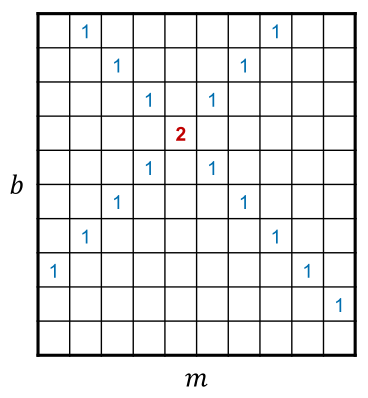
\includegraphics[scale=0.45]{hough_grid.png}
                  	\centering
                  	\caption{hough transform grid}\label{fig:hough_grid}
                \end{figure}
            \item But the parameter space could be too large,
                $[-\infty,+\infty]$; use \emph{normal
                form} instead
                \[
                    x\cos{\theta}+y\sin{\theta}=\rho
                \]
                so at least for one dimension, $\theta\in[0,\pi)$.
        \end{itemize} 
    \item Line detection by Hough transform:
        \begin{enumerate}
            \item Initialize the bins $H(\rho,\theta)$ to all zeros.
            \item For each $(x,y)$ and each $\theta$, calculate $\rho$ and
                $H(\rho,\theta)++$.
            \item Find $(\rho,\theta)$ where $H(\rho,\theta)$ is a local maximum
                and larger than a threshold.
                \begin{itemize}
                    \item local maximum so there can be multiple solutions, to
                        reduce FN
                    \item larger than a threshold so as to reduce FP
                \end{itemize} 
            \item The detected lines are given by
                $\rho=x\cos{\theta}+y\sin{\theta}$.
        \end{enumerate} 
    \item robust to noise/occlusion
        \begin{itemize}
            \item edge map is often generated after image smoothing
            \item broken/unoccluded edge points can still 
                vote and contribute to line detection
        \end{itemize} 
    \item Circle detection by Hough transform
        \begin{itemize}
            \item  parameter space also forms circles
            \item If radius $r$ is also unknown, then 3D parameter space
                $H(a,b,r)$
            \item parameterize to be $x = a+r\cos{\theta}$ and $y =
                b+r\sin{\theta}$, since we know $\theta$ form edge detection, we
                can narrow the voting area to move along $\theta$ for a distance
                $r$.
        \end{itemize} 
    \item Pros and Cons:
        \begin{itemize}
            \item[+] detects multiple instances
            \item[+] robust to image noise
            \item[+] robust to occlusion
            \item[-] Computational complexity is quite high. For each edge
                point, we need to vote to a 2D or even 3D parameter space.
            \item[-] need to carefully set parameters such as those for edge
                detectors, the threshold for the accumulator or range of circle
                radius.
        \end{itemize} 
\end{itemize} 


\section{Interest Point Detection}

\subsection{Definition}

\begin{itemize}
    \item \underline{\textbf{Interest point}}: points that we are interested in
        and are useful for subsequent image processing and analysis.
        They are also called \emph{keypoints}, \emph{landmarks},
        \emph{low-level} features.
\end{itemize} 


\end{document}
